\documentclass[tikz,border=2pt]{standalone}
\usepackage{amsmath}
\usepackage{pgfplots}
\pgfplotsset{compat=1.18}

\begin{document}
% Stationary points are where the tangent is horizontal, f'(x)=0: a local maximum, a local minimum,
% and a point of inflection with f'=0 that is neither.
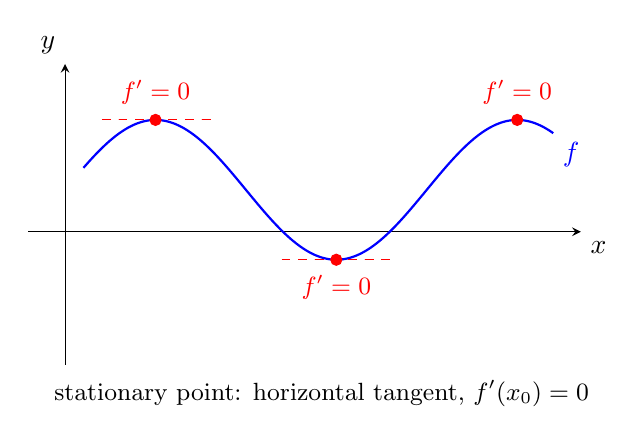
\begin{tikzpicture}
	\begin{axis}[
		axis lines=middle,
		xmin=-0.4, xmax=5.6,
		ymin=-1.9, ymax=2.4,
		xtick=\empty, ytick=\empty,
		xlabel={$x$}, ylabel={$y$},
		xlabel style={below right}, ylabel style={above left},
		samples=200, smooth, clip=false,
		width=8.6cm, height=5.4cm
		]
		% f(x) = 0.5 sin(1.6x) + 0.08(x-4)^3 + 0.6 : stationary points found numerically are approximate
		\addplot[thick, blue, domain=0.2:5.3] {sin(deg(1.6*x))+0.6};
		\addplot[red, dashed, domain=0.4:1.6] {1.6};
		\addplot[red, dashed, domain=2.35:3.55] {-0.4};
		\addplot[only marks, mark=*, red] coordinates {(0.982,1.6) (2.945,-0.4) (4.909,1.6)};
		\node[red, anchor=south, font=\small] at (axis cs:0.982,1.68) {$f'=0$};
		\node[red, anchor=north, font=\small] at (axis cs:2.945,-0.48) {$f'=0$};
		\node[red, anchor=south, font=\small] at (axis cs:4.909,1.68) {$f'=0$};
		\node[blue, anchor=west] at (axis cs:5.3,1.1) {$f$};
	\end{axis}
	\node[anchor=north, font=\small] at ([yshift=-2pt]current axis.outer south) {stationary point: horizontal tangent, $f'(x_0)=0$};
\end{tikzpicture}
\end{document}
